\chapter{Diagrammes Logiciel}
Les prochains diagrammes ont pour but de présenter l'idée de départ de notre architecture logicielle.
En effet, bien que ceci constitue notre architecture visée, cette dernière changera inéluctablement lors du développement, comme le veut la gestion de projet "Agile".
Autre précision, ces diagrammes modélisent seulement les tranches les plus utiles afin d'avoir une bonne vision de l'ensemble du système.

\begin{landscape}
\begin{figure}
  \centering
  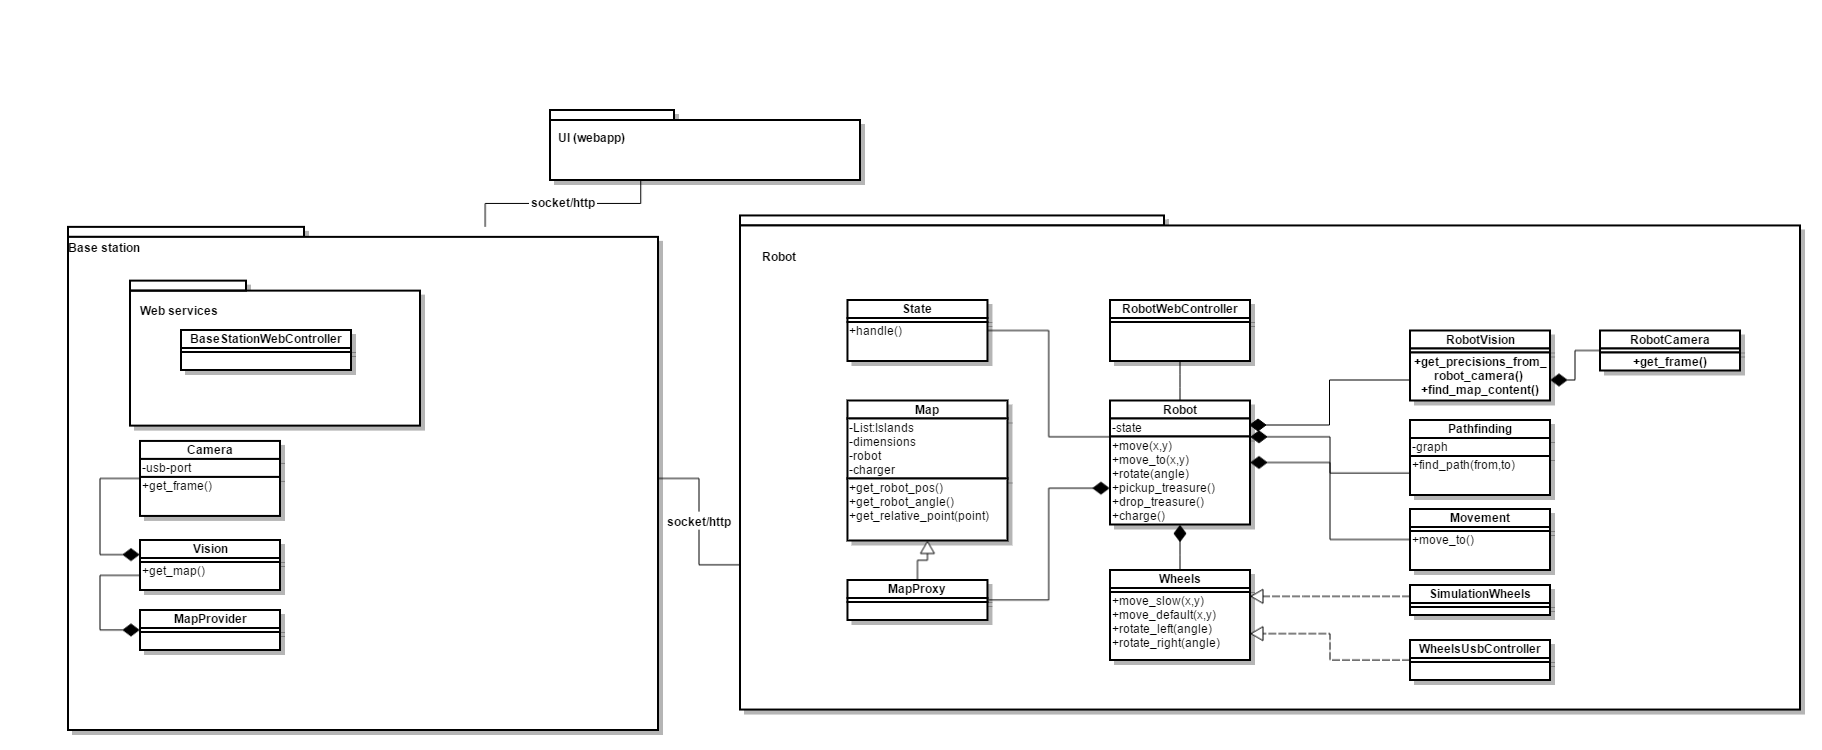
\includegraphics[scale=0.2, angle=0]{resources/diagrams/classDiagram.png}
  \caption{Diagramme de classe}
\end{figure}

\begin{figure}
  \centering
  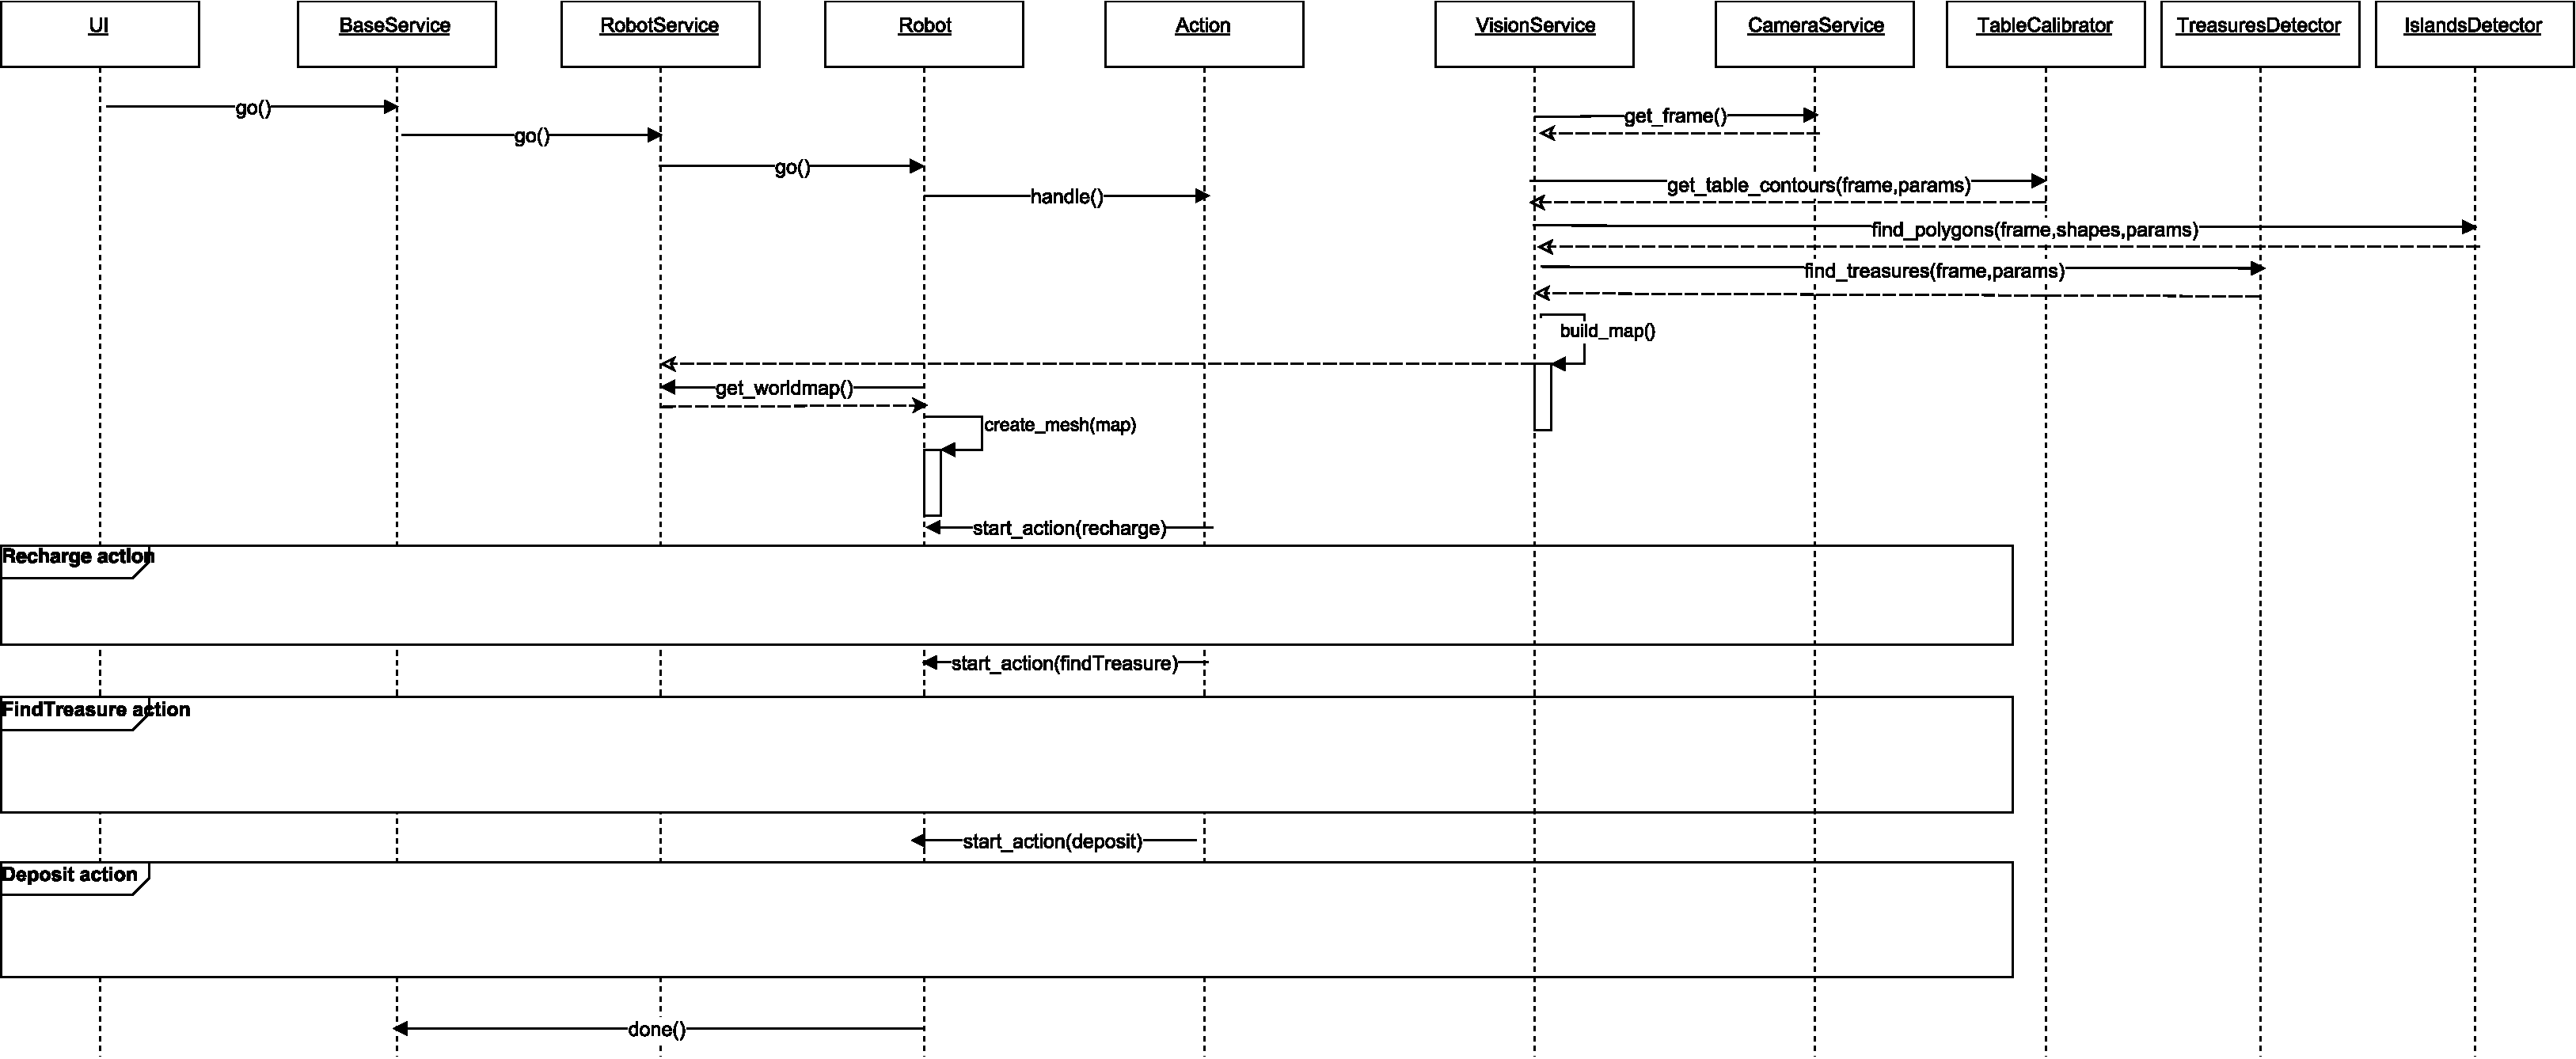
\includegraphics[scale=0.45, angle=0]{resources/diagrams/sequenceDiagram.pdf}
  \caption{Diagramme de séquence complet}
\end{figure}

\begin{figure}
  \centering
  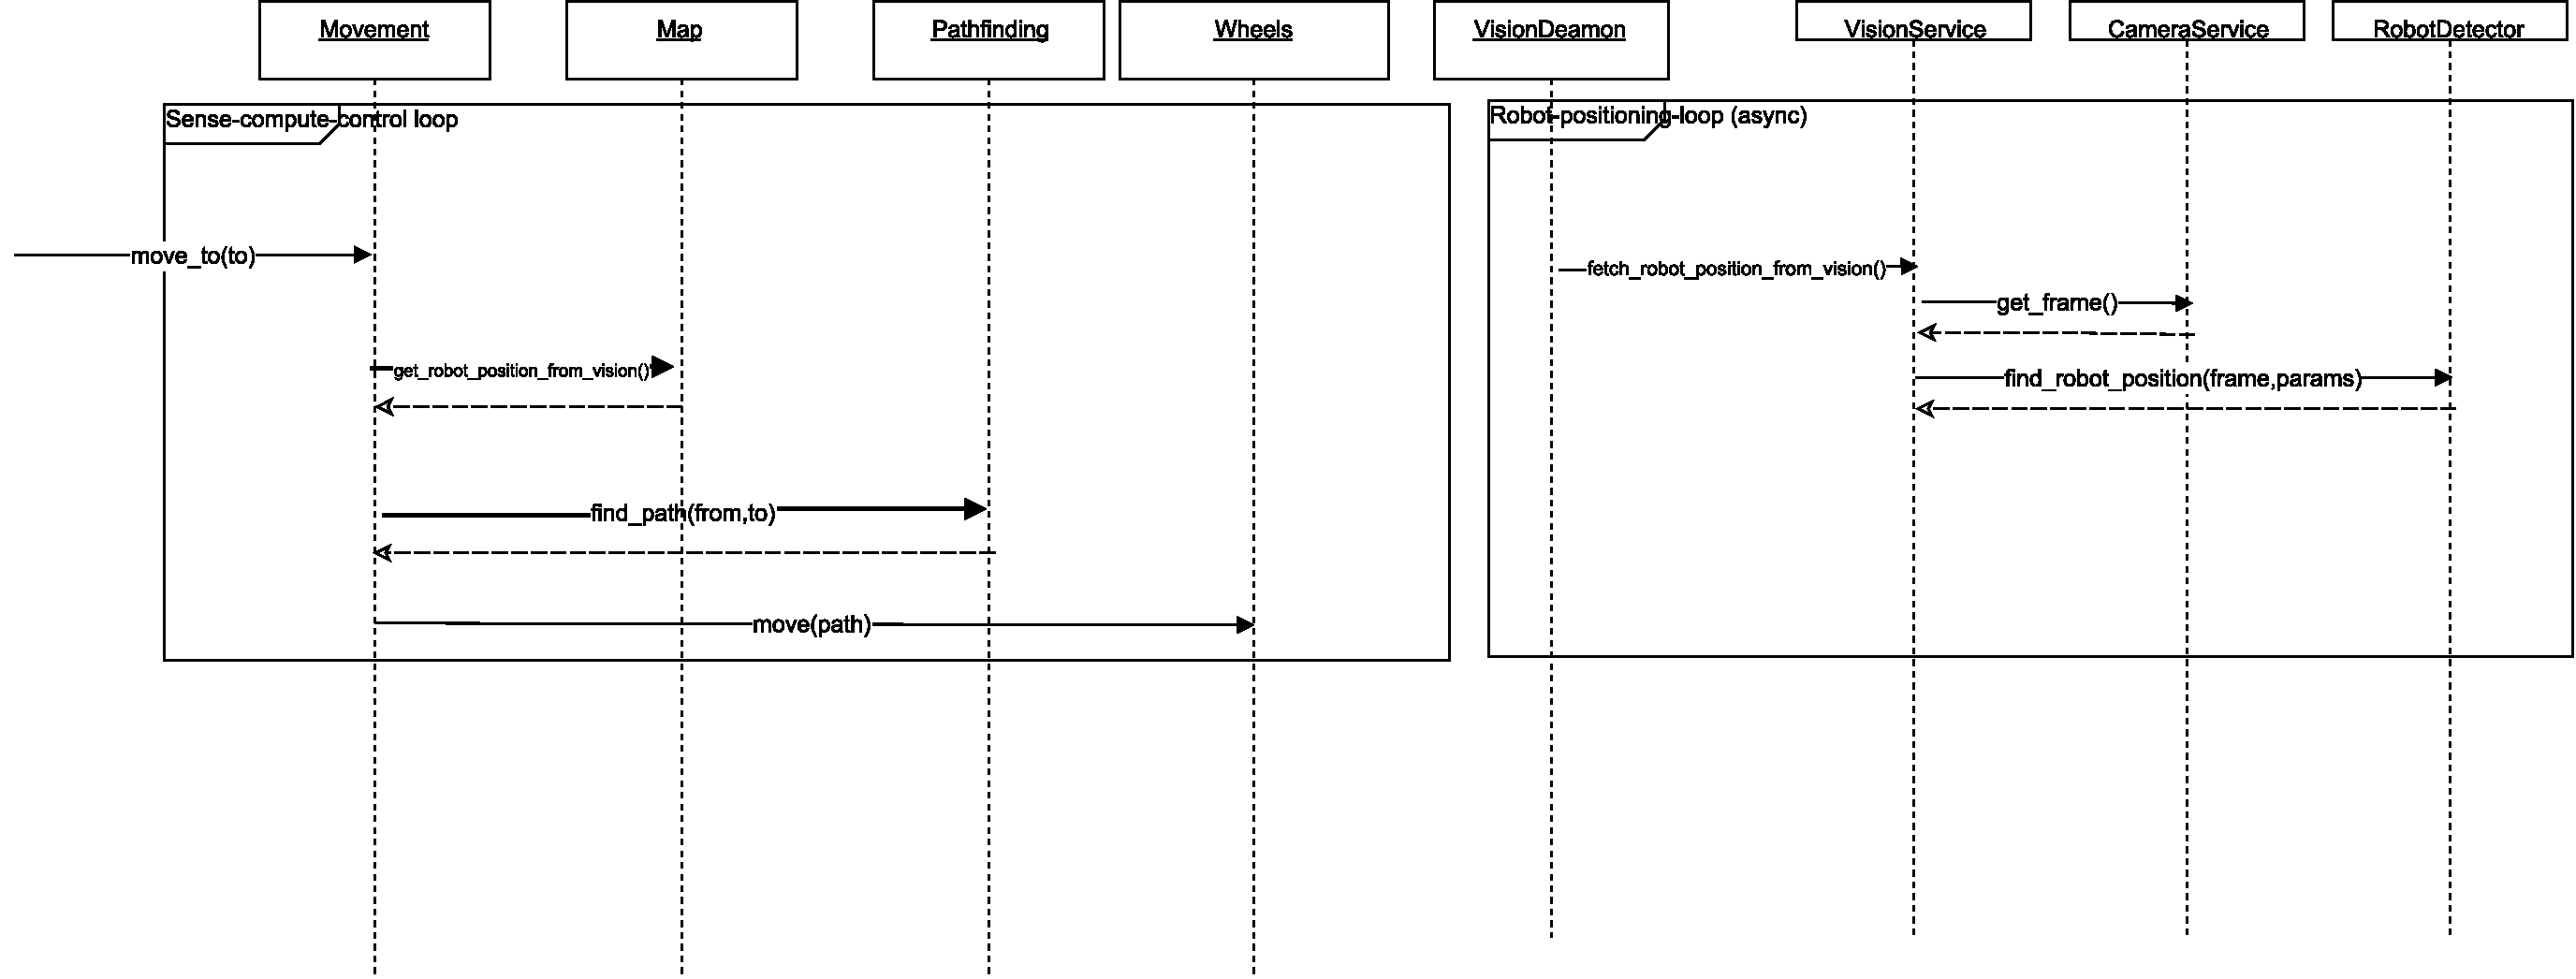
\includegraphics[scale=0.45, angle=0]{resources/diagrams/robotMovement.pdf}
  \caption{Diagramme de séquence de la boucle de sense-compute-control lors d'un déplacement}
\end{figure}

\begin{figure}
  \centering
  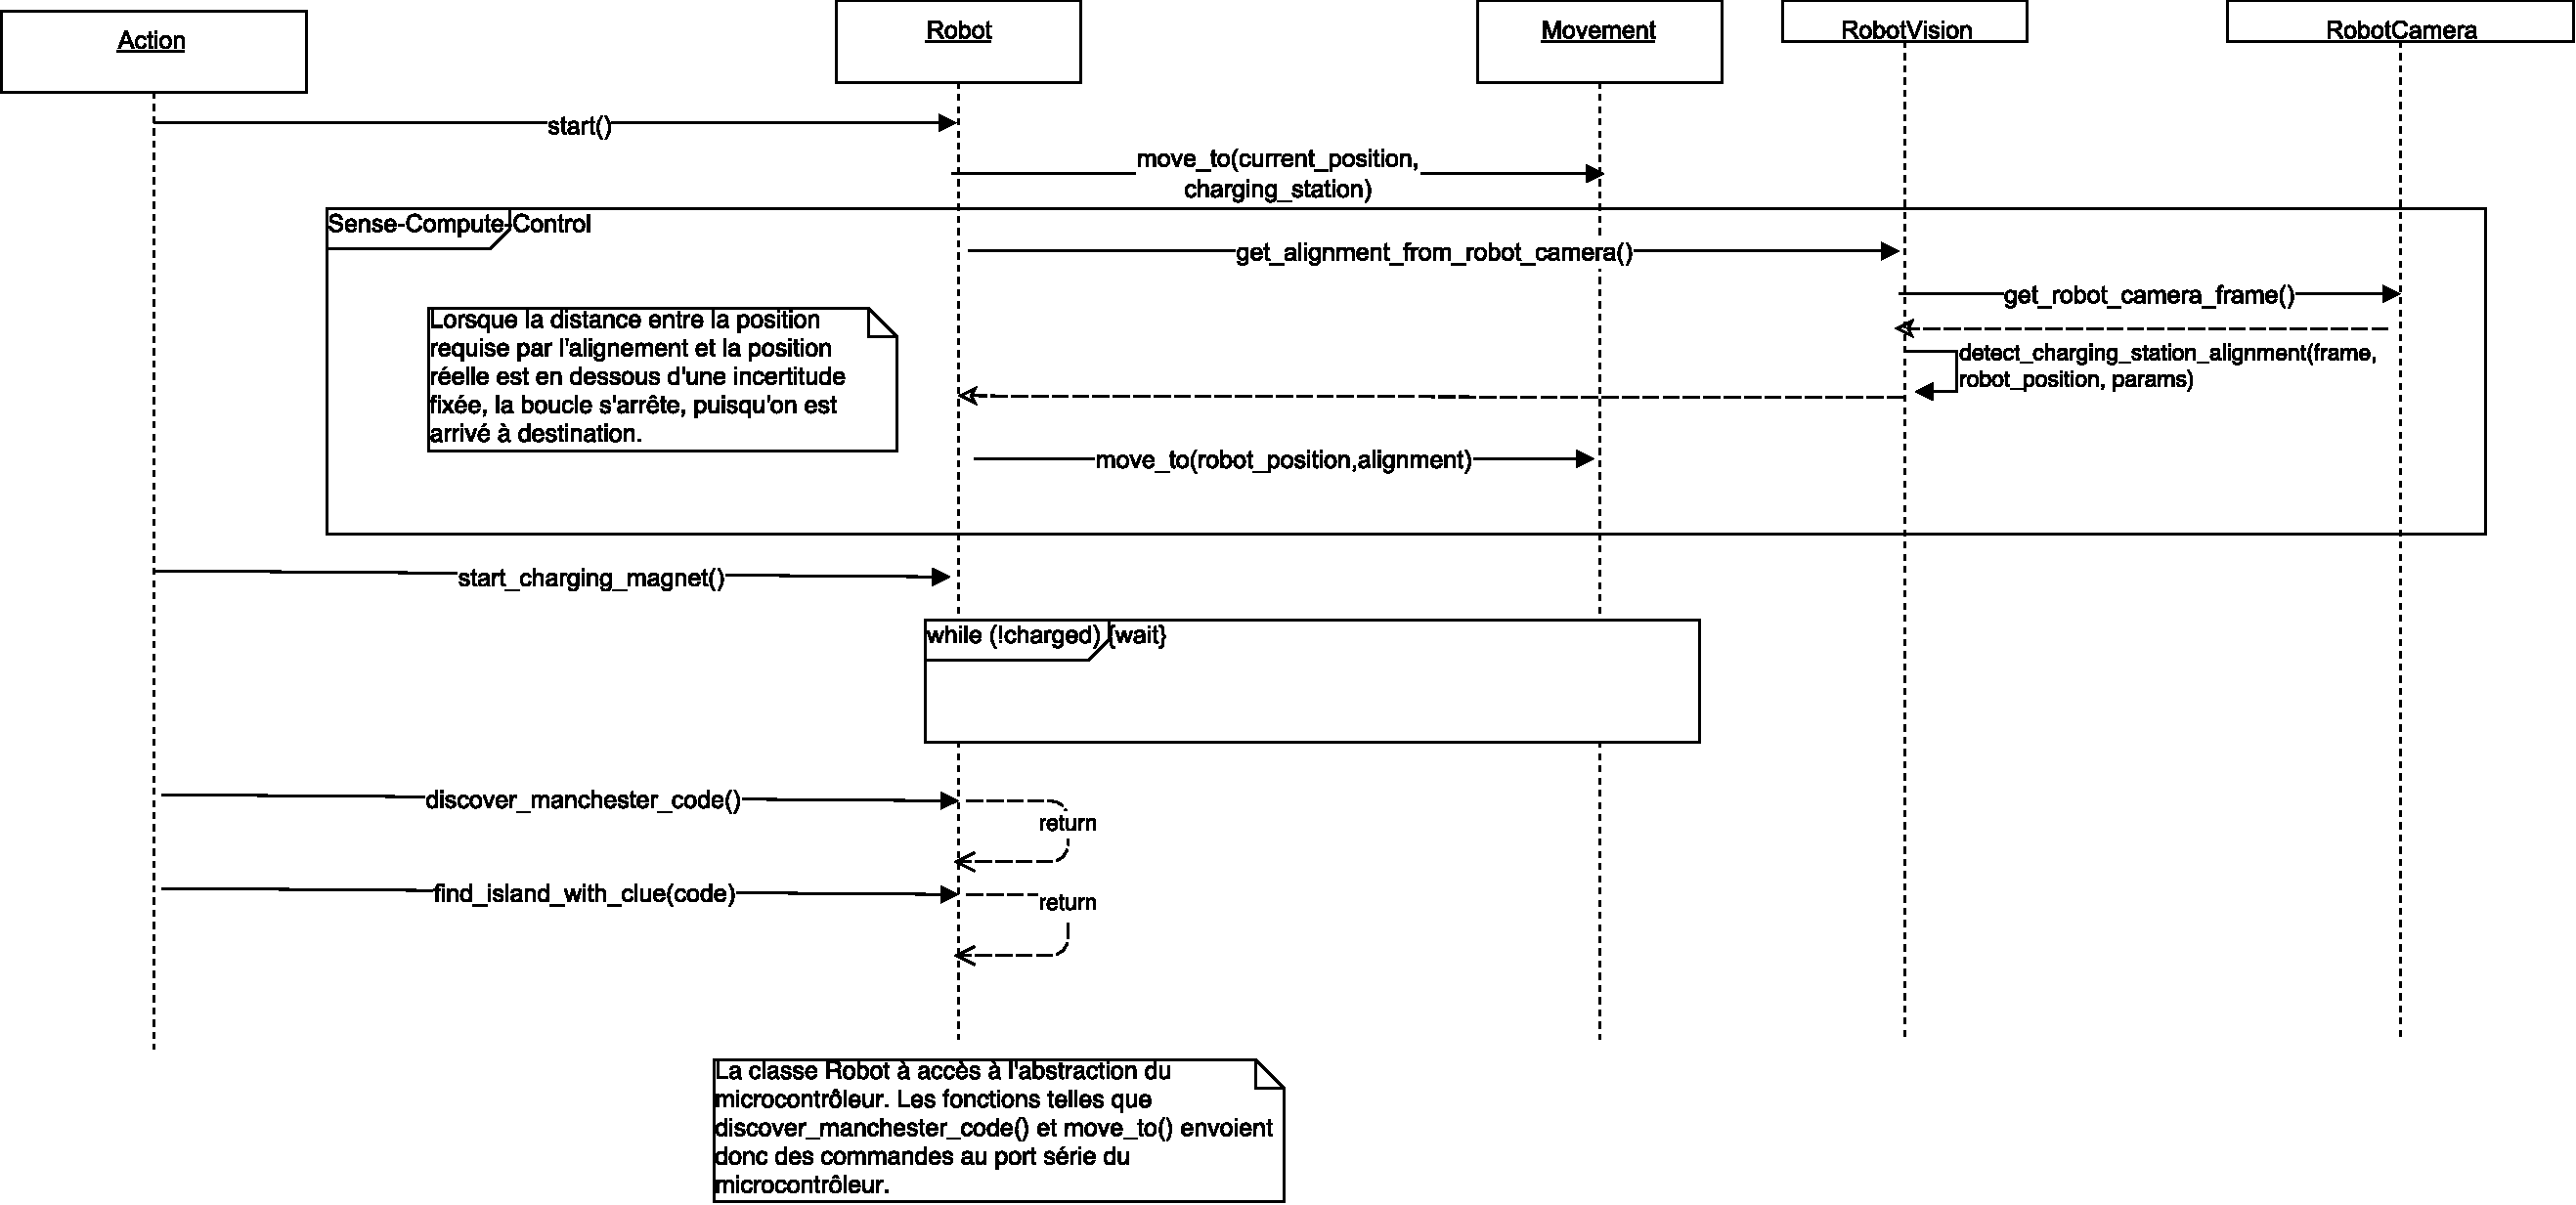
\includegraphics[scale=0.5, angle=0]{resources/diagrams/rechargeAction.pdf}
  \caption{Diagramme de séquence de recharge}
\end{figure}

\begin{figure}
  \centering
  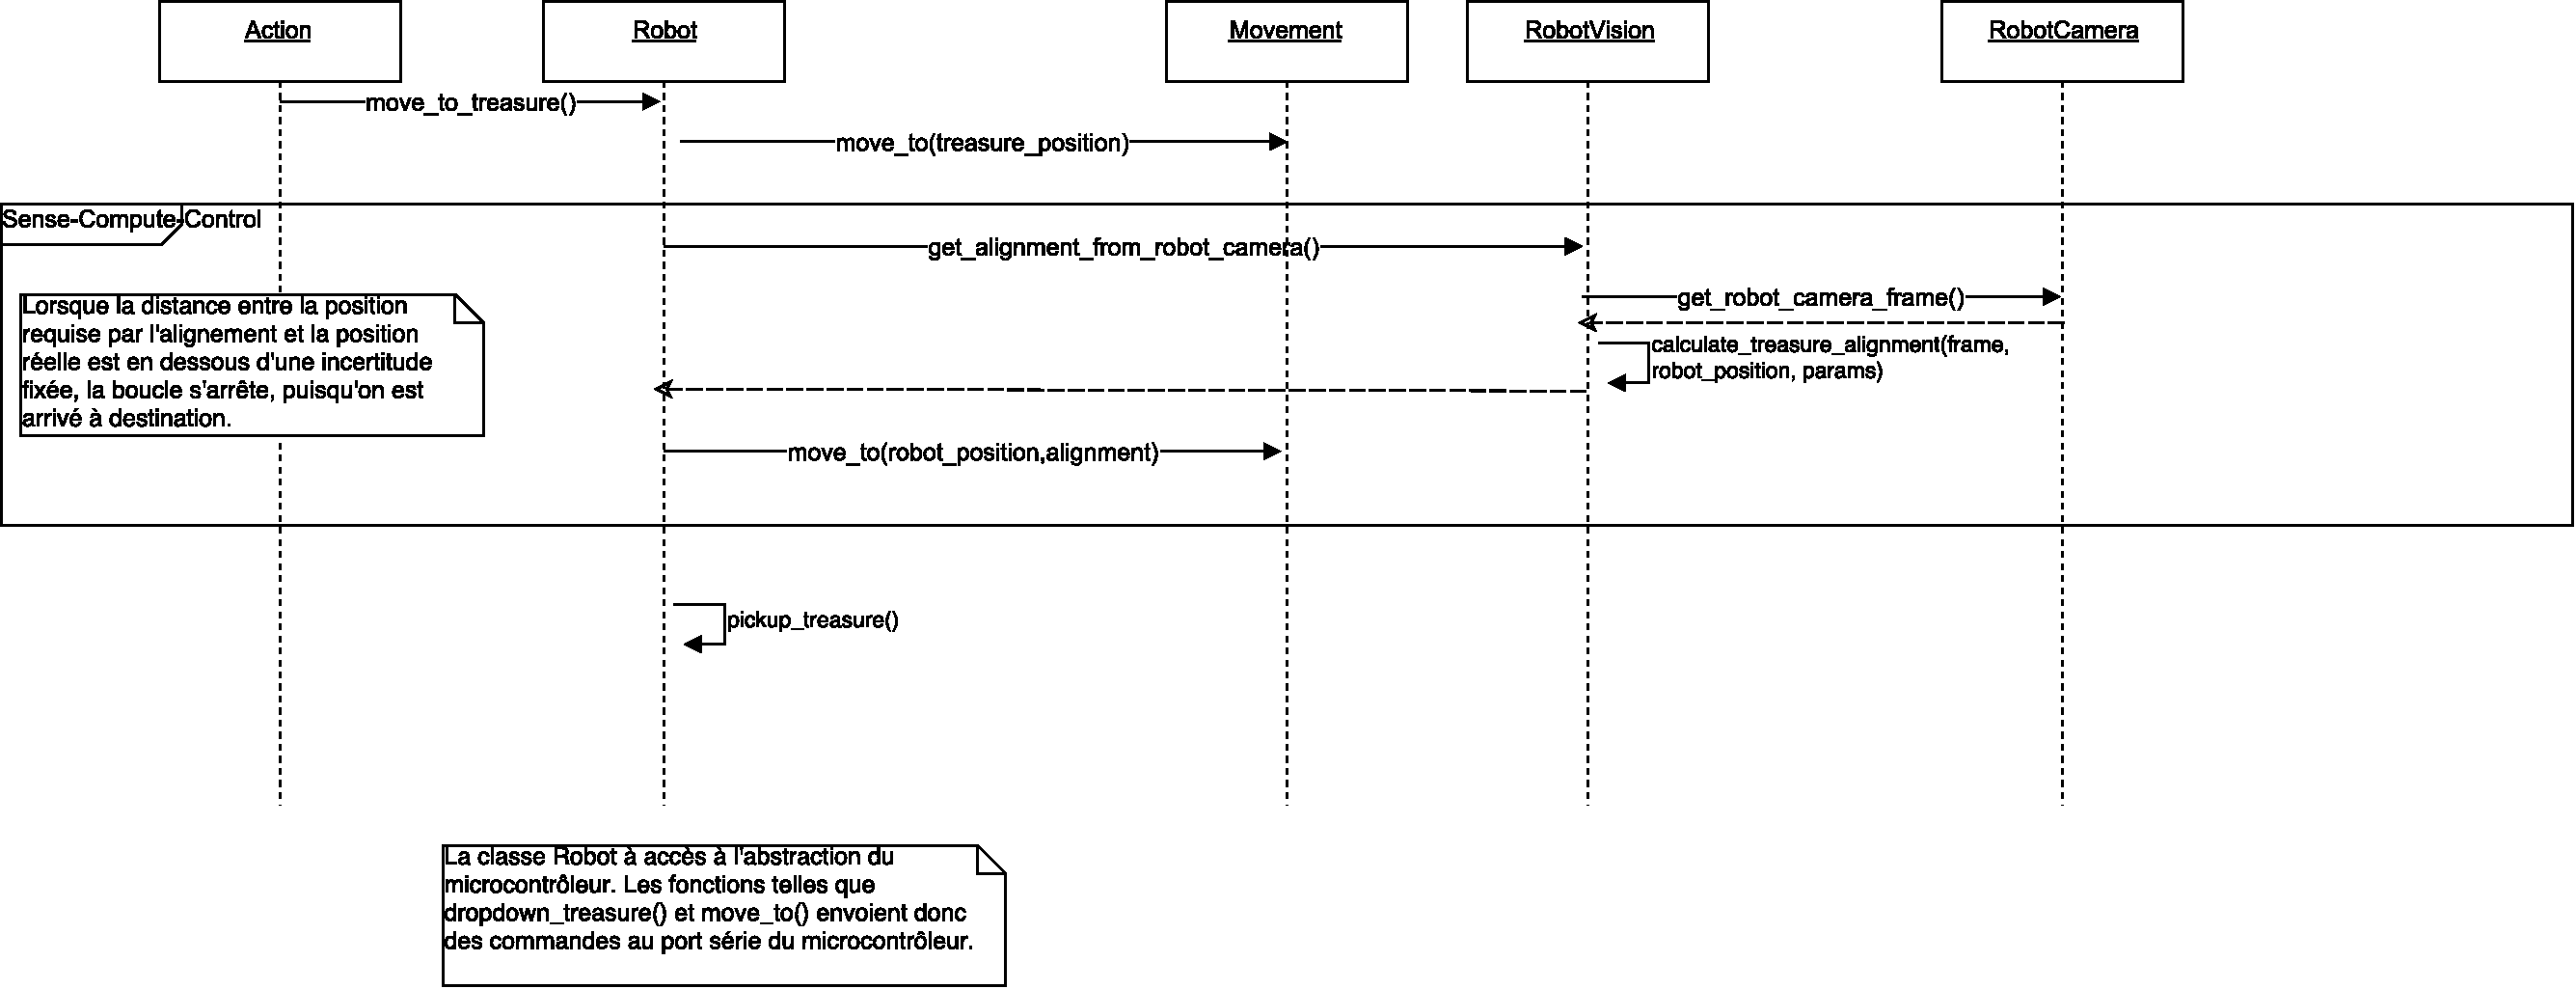
\includegraphics[scale=0.4, angle=0]{resources/diagrams/findTreasureAction.pdf}
  \caption{Diagramme de séquence de recherche de trésor}
\end{figure}

\begin{figure}
  \centering
  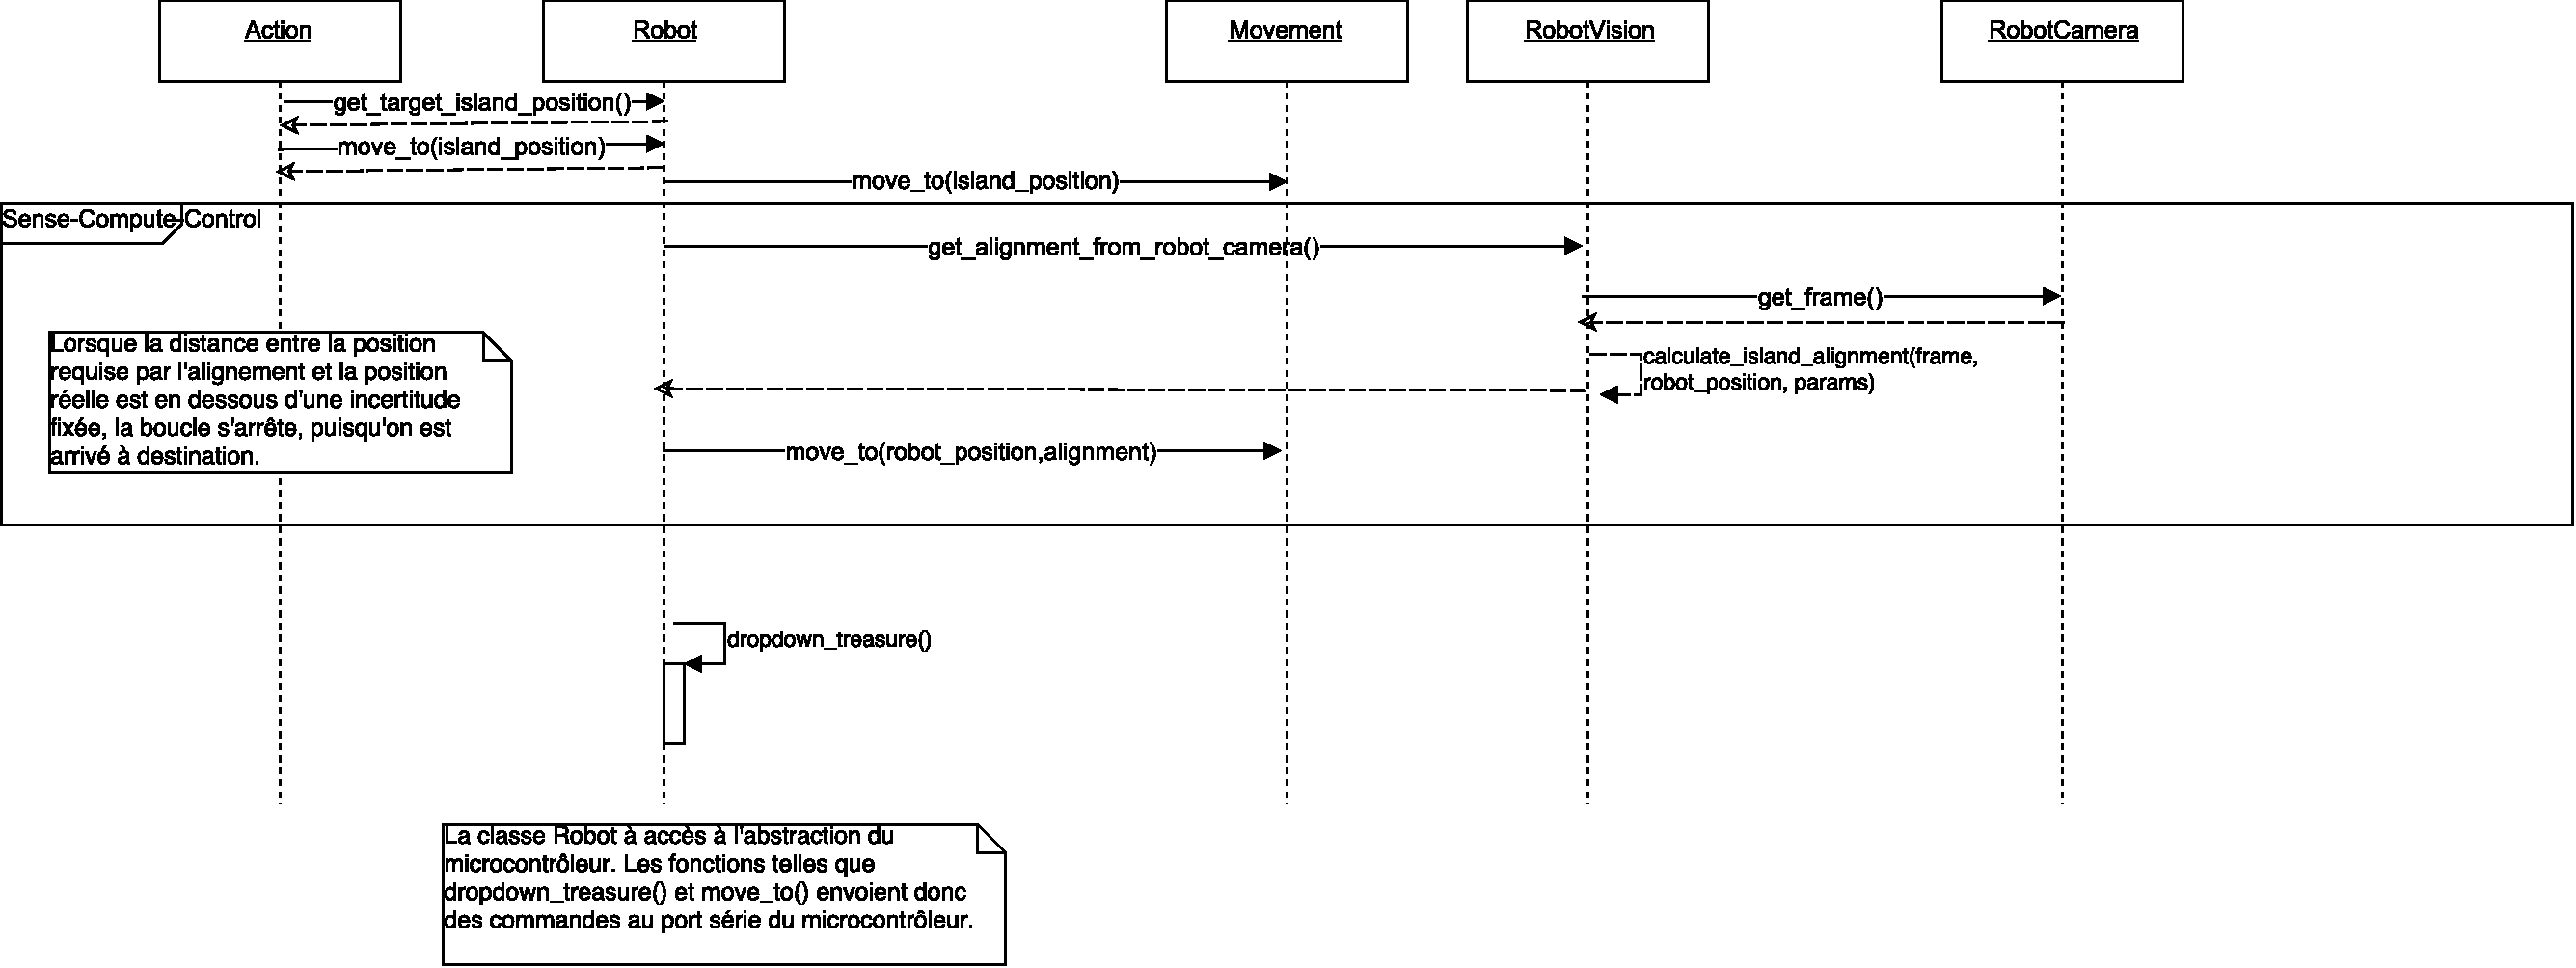
\includegraphics[scale=0.5, angle=0]{resources/diagrams/depositAction.pdf}
  \caption{Diagramme de séquence dépot du trésor}
\end{figure}
\end{landscape}
